\documentclass[a4paper,twoside]{article}

%% Language and font encodings
\usepackage[spanish]{babel}
\usepackage[utf8]{inputenc}
\usepackage[T1]{fontenc}


%% Sets page size and margins
\usepackage[a4paper,top=3cm,bottom=2cm,left=2.5cm,right=2.5cm,marginparwidth=0.5cm]{geometry}

\usepackage{amsmath}			%Paquete matemático
\usepackage{graphicx}
\usepackage[colorinlistoftodos]{todonotes}

\usepackage{hyperref}		%Paquete empleado para colocar hipervinculos
\hypersetup{
	colorlinks = true,
	linkcolor = black,
}

\usepackage{eurosym}
\usepackage{pdfpages}			%Sirve para incluir PDF en el documento
\usepackage{anysize}			%Podremos colocar imagenes de cualquier tamaño
\usepackage{subfig}				%Nos permitira colocar varias imagenes en una figura
\usepackage{float}				%Podremos crear y colocar boxes donee queramos
\usepackage[export]{adjustbox}

%Colocamos cabeceras y pies de pagina
%(CONSULTA: http://edicionesoniricas.com/maquetar-latex-encabezados-pies-pagina/)
%(CONSULTA2: https://es.sharelatex.com/learn/Headers_and_footers)
%\bfseries es análogo a \textbf{}
% \leftmark-> Adds name and number of the current top-level structure (section for article) in uppercase letters.
%\rightmark-> Adds name and number of the current next to top-level structure (subsection for article) in uppercase letters.
\usepackage{fancyhdr}		%Paquetes necesarios
\pagestyle{fancy}			%Borra los parametros por defecto
\fancyhf{}
\fancyhead[RO,LE]{\bfseries\thepage}
\fancyhead[LO,RE]{\bfseries\rightmark}
%Nos aseguramos de que en las paginas plain, no haya ni cabeceras ni lineas
\fancypagestyle{plain}
{
	\fancyhead{} % elimina cabeceras en paginas "plain"
	\renewcommand{\headrulewidth}{0pt} % así como la raya
}

%Definimos las lineas divisoras de las cabeceras y pie de pagina
\renewcommand{\headrulewidth}{1pt}	%Define el grosor de la línea de head
\renewcommand{\footrulewidth}{0pt}		%Define el grosor de la linea foot (Si no queremos linea, 0pt)
\addtolength{\headheight}{0.5pt} % espacio para la raya

%Librerias para introducir código de Matlab
%\usepackage{bigfoot} % to allow verbatim in footnote
\usepackage[numbered,framed]{matlab-prettifier}

\lstset{
	style              = Matlab-editor,
	basicstyle         = \mlttfamily,
	escapechar         = ",
	mlshowsectionrules = true,
}

% Pie de pagina
%\fancyfoot{} % limpia el pie
\fancyfoot[C]{- \thepage -} % número de página centrado

%Nos generará texto para pruebas de maquetado
\usepackage{lipsum}

% Se varia el limite de colimnas de latex
\setcounter{MaxMatrixCols}{11}
\usepackage{lscape}
%----------------------------------------------------------------------------------------------------------------------------------
\begin{document}
\begin{titlepage}
	\centering
\Huge{\textbf{CONTROL Y PROGRAMACIÓN DE ROBOTS}} \\
\Huge{\textit{Proyecto de robótica móvil}}\\

\vspace{1cm}
\LARGE{Grado en Ingeniería Electrónica, Mecatrónica y Robótica}\\
\rule{\textwidth}{0.1mm}
%  %%%%% Este trozo de codigo es para insertar imagenes %%%%%%%
\begin{figure}[h!]
	\centering
	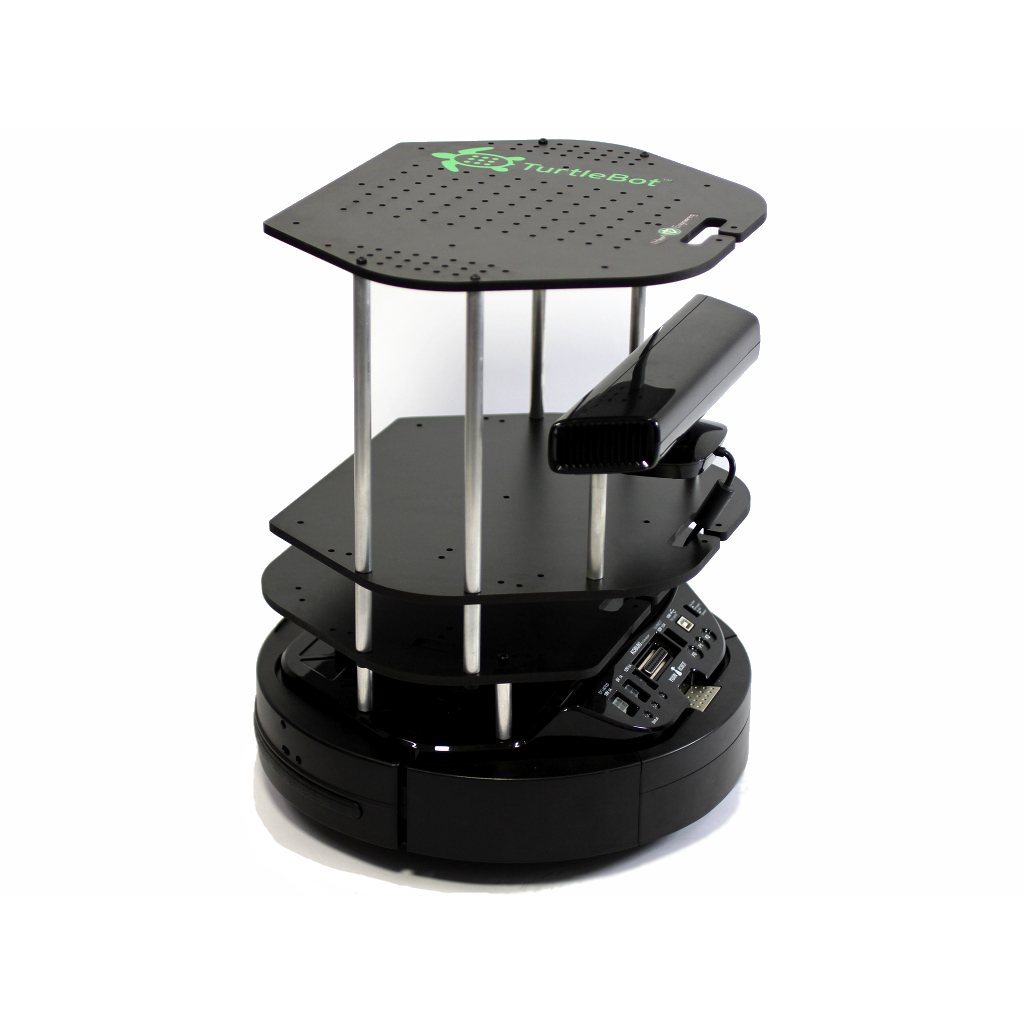
\includegraphics[width=.7\textwidth]{robot_portada}
	%\caption{textodelaleyenda}
\end{figure}
% %%%%%%%%%%%%%%%%%%%%%%%%%%%%%%%%%%%%%%%%%%%%%%%%%%%%%%%%%%%%%
\vspace{1cm}
\rule{\textwidth}{0.1mm}
\Large{\textbf{Autores:} Montes Grova, Marco Antonio\\
 Lozano Romero, Daniel\\
 Mérida Floriano, Javier}
\end{titlepage}
\tableofcontents
\newpage
% %%%%%%%%%%%   INTRODUCCION %%%%%%%%%%%%%%%%%%
\section{Introducción al proyecto}
En el proyecto que sigue a continuación se desarrollará el modelado y control de un robot móvil tipo síncrono. La principal característica destacable de este tipo de robots recae en el mecanismo mecánico interno que posee mediante el cuál se podrán mover 3 ruedas empleando únicamente 2 motores.\\
Con uno de los motores se desplazará en línea recta y con el otro se le dará el ángulo de giro deseado sobre sí mismo.\\

El modelo síncrono se basa en 3 ruedas idénticas que se desplazan y giran al unísono, haciendo posible que el robot pueda moverse en cualquier dirección y orientación en el plano del suelo. Estas ruedas están dispuestas de forma triangular en la base del robot, el cual se va a representar como un objeto cilíndrico, siendo la base uno de los lados circulares.\\

Este modelo tiene como ventajas la separación de motores entre traslación y rotación que facilita el control, la garantía de control en trayectorias rectilíneas debido a la mecánica del mismo y la facilidad que incluyen las restricciones homólogas que posee. Como desventaja encontramos el complejo diseño mecánico que posee para poder transmitir la rotación y traslación a las tres ruedas simultáneamente y, por ende, su difícil implementación en la realidad.\\
% SEGUIR HABLANDO DE MOVIDAS TEORICAS UN PSEUDO LARGO TRECHO ETC ETC ETC ETC



\section{Análisis cinemático}
	\subsection{Obtención del modelo cinemático directo y su Jacobiano}
	Gracias a la mecánica del modelo síncrono, los cálculos para la obtención del modelo cinemático del mismo van a ser muy sencillos, ya que se trata de un modelo con restricciones holónomas, es decir, el comportamiento del vehículo se puede representar a través de sus variables generalizadas ($x$ e $y$ como coordenadas del centro del robot en el plano del suelo y $\varphi$ como la rotación producida frente al estado inicial, es decir, cuando éste vale cero) y la variable temporal y puede ser integrable, simplificando el cálculo.\\
	
	Para el modelo cinemático en cuestión, sólo se necesita como dato el valor del radio de las ruedas, $R$, para poder realizar la conversión entre velocidad angular y velocidad lineal. En este trabajo, siendo el grupo de trabajo número 11, se tiene cómo radio de las ruedas el valor de $R = 0.4 m$. Con esto ya se puede hallar el modelo cinemático del robot:\\
	
	Para comenzar se deben detectar las variables generalizadas y de actuación del sistema, respectivamente:
		$$
		q=
		\begin{bmatrix}
		x\\y\\\varphi
		\end{bmatrix}
		$$		
		{\centering y \par}
		$$
		p=
		\begin{bmatrix}
		\dot{\theta}\\\omega
		\end{bmatrix}
		$$

	Como ya se sabe de clase, las variables generalizadas son las que dan información sobre el estado del robot, ya que se encuentran en ellas las coordenadas cartesianas $x$ e $y$ del plano del centro del robot y el ángulo de giro $\varphi$ con respecto al eje X, como se ha decidido definir en este proyecto. Así mismo, las variables de actuación son, como dice su nombre, las variables que reflejarán el valor de movimiento de los motores del robot, es decir, del motor de desplazamiento (velocidad angular $\dot{\theta}$) y el de rotación (velocidad angular $\omega$).\\
	
	Una vez detectadas las variables del sistema, se debe encontrar la relación entre ellas y así conseguir la expresión del Jacobiano:\\
	
	Primero, se define $v$ como la componente global de velocidad de desplazamiento, por lo que se calculará como $v^2=\dot{x}^2+\dot{y}^2$ o como $v=R \dot{\theta}$ y, a su vez, la componentes cartesianas de la velocidad se definirán como\par
	
	{\centering $\dot{x}=v cos(\varphi)$\par} {\centering $\dot{y}=v sin(\varphi)$\\}
	
		
	Sabiendo además que la velocidad de rotación $\dot{\varphi}$ concuerda con la variable de actuación $\omega$, se puede montar la matriz Jacobiana del sistema tal que:
		$$
		J=
		\begin{bmatrix}
			R cos(\varphi) && 0\\
			R sin(\varphi) && 0\\
			0 && 1
		\end{bmatrix}
		$$

	La matriz Jacobiana describirá la cinemática del sistema relacionando las variables de actuación con las derivadas de las variables generalizadas y, como se sabe que serán integrables debido a la existencia de restricciones holónomas, se podrán integrar para poder hallar los valores de posición y orientación.\\
	
	Dicho esto, se puede expresar el modelo cinemático como función de entradas (variables de actuación) y salidas (variables generalizadas):
	
		$$
		\begin{bmatrix}
		\dot{x}\\\dot{y}\\\dot{\varphi}
		\end{bmatrix}
		=
		\begin{bmatrix}
		R cos(\varphi) && 0\\
		R sin(\varphi) && 0\\
		0 && 1
		\end{bmatrix}
		\begin{bmatrix}
		\dot{\theta}\\\omega
		\end{bmatrix},
		$$

	e integrando,
	
		$$
		\begin{bmatrix}
		x\\y\\\varphi
		\end{bmatrix}
		=
		\begin{bmatrix}
		x_0\\y_0\\\varphi_0
		\end{bmatrix}
		+
		\begin{bmatrix}
		\int_{0}^{t} R\dot{\theta}cos(\varphi)dt\\
		\int_{0}^{t} R\dot{\theta}sin(\varphi)dt\\
		\int_{0}^{t} \omega dt
		\end{bmatrix},
		$$
	
	siendo $x_0$, $y_0$ y $\varphi_0$ las condiciones iniciales de posición y orientación.


	\subsection{Obtención del modelo cinemático inverso}
	\subsection{Definición de las trayectorias de lazo abierto del robot}
		\subsubsection{Verificación de la actuación senoidal}

\section{Control dinámico}
	\subsection{Implementación de diversos algoritmos de control}
		\subsubsection{Control a un punto}
		\subsubsection{Control a una linea}
		\subsubsection{Control a una trayectoria}
		\subsubsection{Control a una postura}
	\subsection{Ley de control \textit{Persecución pura}}

\section{Anexos y conclusiones}
\end{document}
